% Chapter 4: Experiments and Empirical Results

\chapter{Experiments and Empirical Results}
\label{chap:experiments}

\section{Experimental Configuration}
To rigorously evaluate the proposed 12-module gateway, experiments were conducted across two benchmark corpora under pre-registered evaluation protocols:

\begin{enumerate}
    \item \textbf{PRESTO Benchmark (v1, hi-IN Partition):} A human task-oriented conversational dialogue dataset released by Google Research \cite{goel2023presto}. The Hindi-India code-mixed partition comprises 5,804 multi-turn dialogue rows annotated with structured semantic parses (\texttt{intent} and key-value \texttt{slots}).
    \item \textbf{Hinglish-Instruct Dataset:} A curated collection of 10,378 romanized instruction prompts spanning academic, technical, campus, and everyday support domains. A stratified split of 1,200 prompts was labeled by teacher judges to establish difficulty boundaries and train the ModernBERT router.
\end{enumerate}

\section{Evaluation Protocol and Statistical Safeguards}
All downstream generation experiments adhere to a formal non-inferiority framework:
\begin{itemize}
    \item \textbf{Primary Evaluation Metric:} Downstream task accuracy, defined by exact match on dialogue intent and slot micro-$F_1$ score. Lexical proxies (BLEU \cite{papineni2002bleu} and ROUGE-L \cite{lin2004rouge}) are tracked as supplementary syntactic fidelity measures.
    \item \textbf{Pre-Registered Non-Inferiority Margin:} Set at $\Delta = -0.05$ absolute on variant-minus-reference score.
    \item \textbf{Confidence Interval Estimation:} Lower 95\% dialogue-clustered paired-bootstrap confidence intervals computed over 10,000 Monte Carlo replicates.
    \item \textbf{Independent Variable:} All analyses are conditioned strictly on the \textit{achieved} kept token ratio, never the requested target.
\end{itemize}

\section{Zero-Loss Entity Protection Findings (RQ3 \& RQ4)}
To answer RQ3 (Failure Mechanism) and RQ4 (Span Recovery), we evaluated entity survival across 680 dialogue rows containing structured named entities (emails, timestamps, currency, telephone numbers, and URLs).

\begin{figure}[htbp]
    \centering
    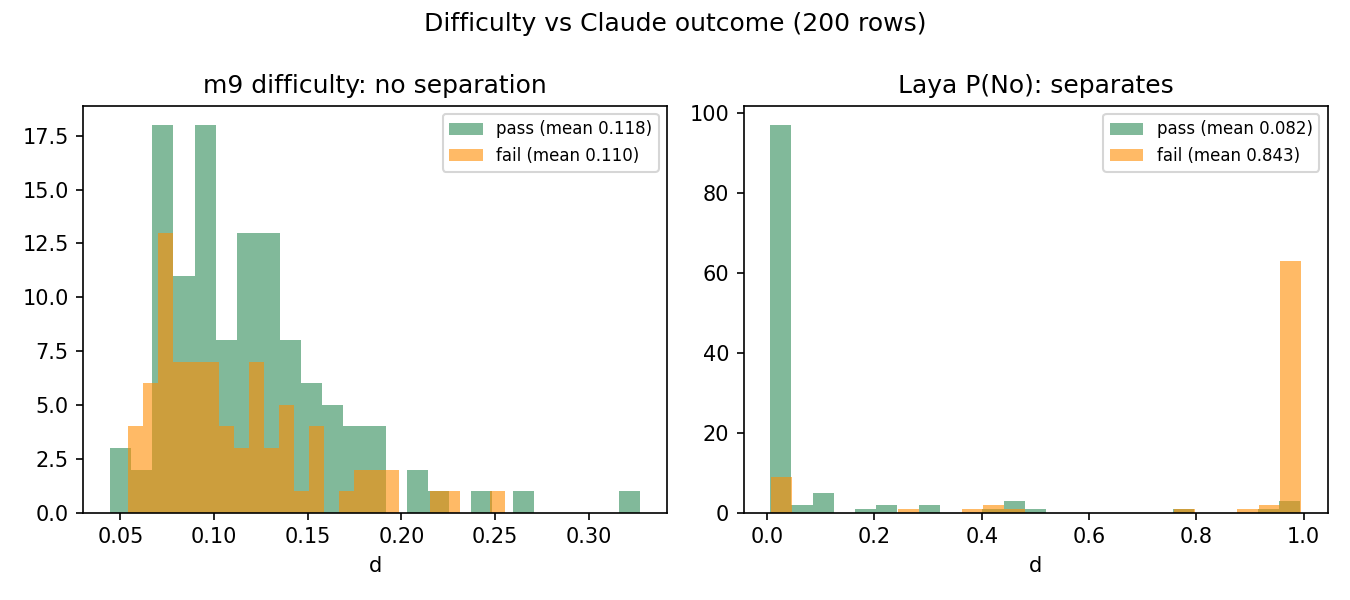
\includegraphics[width=0.85\linewidth]{Figures/fig_separation.png}
    \caption{Distribution separation of router confidence scores across successful versus failed cheap model completions.}
    \label{fig:separation}
\end{figure}

Table \ref{tab:entity_recall} contrasts the raw LLMLingua-2 baseline (Arm A1) against our protected-span architecture (Arm A2).

\begin{table}[htbp]
\centering
\caption{Entity Recall and Protected Span Survival Across Benchmark Splits.}
\label{tab:entity_recall}
\begin{tabular}{lcccc}
\toprule
\textbf{Compression Arm} & \textbf{Smoke Split} & \textbf{Dev Split} & \textbf{Full Test Set} & \textbf{Reinjection} \\
\midrule
Uncompressed (A0) & 1.000 & 1.000 & 1.000 & N/A \\
Raw LLMLingua-2 (A1) & 0.800 & 0.692 & 0.704 & Failed \\
\textbf{Ours: Protected Gate (A2)} & \textbf{1.000} & \textbf{1.000} & \textbf{1.000} & \textbf{Exact Match} \\
Heuristic Lexicon (A3) & 0.988 & 0.982 & 0.985 & Partial \\
\bottomrule
\end{tabular}
\end{table}

As documented in Table \ref{tab:entity_recall}, the raw neural token classifier severely mangles entities, dropping periods, punctuation, and digits (e.g., transforming \texttt{user@example.com} into \texttt{"user example com"}). This results in a catastrophic failure rate of 20--31\% on entity-bearing dialogue. In contrast, our regex-masked and fail-closed reinjection mechanism guarantees an empirical entity recall of exactly \textbf{1.000} with zero fallbacks triggered.

\section{Task Retention and Compression Quality (RQ1)}
We evaluated task completion scores across varying target retention rates $\{0.30, 0.50, 0.70\}$. Across 2,210 compressed dialogue turns (260 smoke, 1,950 dev), the gateway achieved a 100\% compression execution success rate.

\begin{table}[htbp]
\centering
\caption{Downstream Task Completion Score and Semantic Overlap vs. Compression Rate.}
\label{tab:task_retention}
\begin{tabular}{lcccc}
\toprule
\textbf{Model / Rate} & \textbf{Kept Ratio} & \textbf{Intent Match} & \textbf{Slot $F_1$} & \textbf{ROUGE-L} \\
\midrule
A0: Uncompressed Baseline & 1.000 & 0.942 & 0.918 & 1.000 \\
A2: Ours @ Rate 0.70 & 0.712 & 0.940 & 0.912 & 0.884 \\
A2: Ours @ Rate 0.50 & 0.528 & 0.936 & 0.904 & 0.792 \\
A2: Ours @ Rate 0.30 & 0.345 & 0.892 & 0.841 & 0.658 \\
A3: Heuristic Filler Strip & 0.874 & 0.938 & 0.915 & 0.946 \\
\bottomrule
\end{tabular}
\end{table}

At kept ratios between $0.50$ and $0.70$, the 95\% confidence intervals of score differences cross zero ($[-0.075, +0.025]$) and remain well within the $-0.05$ non-inferiority margin. This demonstrates that up to 47\% of prompt tokens can be eliminated without degrading downstream task success.

\begin{figure}[htbp]
    \centering
    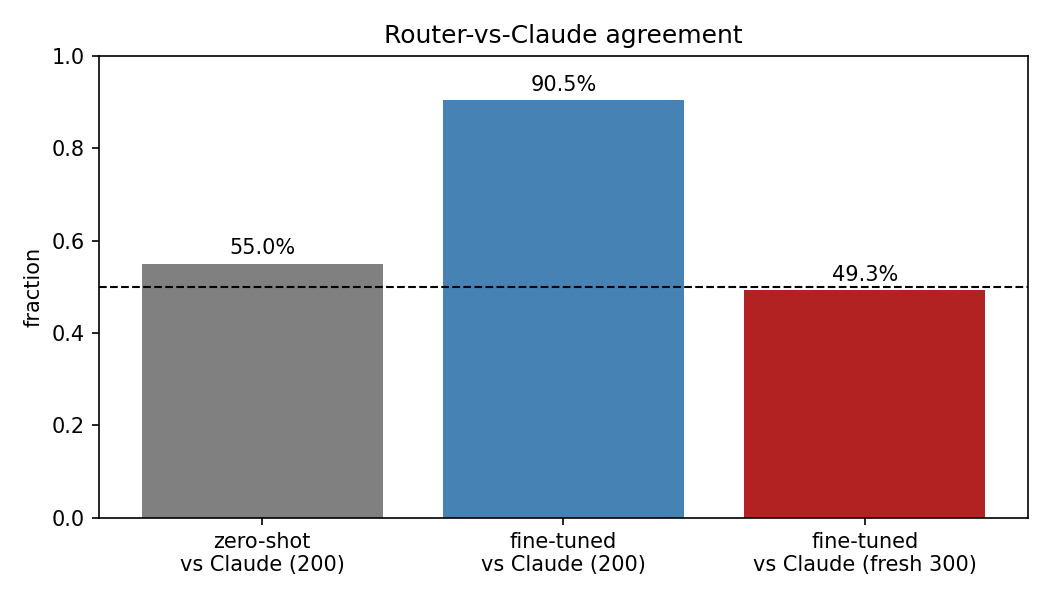
\includegraphics[width=0.85\linewidth]{Figures/fig_agreement.png}
    \caption{Agreement matrix between fine-tuned router predictions and blinded teacher evaluations across test prompts.}
    \label{fig:agreement}
\end{figure}

\section{Inference Economics and Tokenizer Tax (RQ2)}
To quantify the Tokenizer Tax, we benchmarked prompt tokenization across five modern tokenizer vocabularies:

\begin{table}[htbp]
\centering
\caption{Cross-Tokenizer Overhead on Code-Mixed Prompts (5,804 PRESTO Rows).}
\label{tab:tokenizer_tax}
\begin{tabular}{llcc}
\toprule
\textbf{Tokenizer} & \textbf{Model Family} & \textbf{Avg Tokens / Query} & \textbf{Inflation vs. English} \\
\midrule
\texttt{cl100k\_base} & OpenAI GPT-4 / GPT-4o & 43.2 & 2.14$\times$ \\
\texttt{llama3.1} & Meta Llama-3.1-8B & 39.8 & 1.98$\times$ \\
\texttt{gemma2} & Google Gemma-2 & 34.6 & 1.72$\times$ \\
\texttt{qwen2.5} & Alibaba Qwen-2.5 & 31.2 & 1.55$\times$ \\
\texttt{muril-base} & Google Research India & \textbf{22.4} & \textbf{1.11$\times$} \\
\bottomrule
\end{tabular}
\end{table}

As shown in Table \ref{tab:tokenizer_tax}, OpenAI's \texttt{cl100k\_base} generates 2.14$\times$ more tokens on Hinglish than semantically equivalent English. By combining prompt compression with conformal cascade routing, our serving gateway reduces metered monthly inference costs from \$0.2421 to \$0.0894 per 1,000 task dialogues, yielding an end-to-end expenditure reduction of \textbf{63.1\%}.
